% Full pipeline diagram for Go binary decompilation project.
% Compile standalone or \input{} into a larger document.
%
% Dependencies: tikz, tikz libraries (shapes, arrows.meta, positioning, fit, calc, backgrounds)

\documentclass[border=10pt]{standalone}
\usepackage[T1]{fontenc}
\usepackage{tikz}
\usetikzlibrary{shapes.geometric, arrows.meta, positioning, fit, calc, backgrounds}

\begin{document}

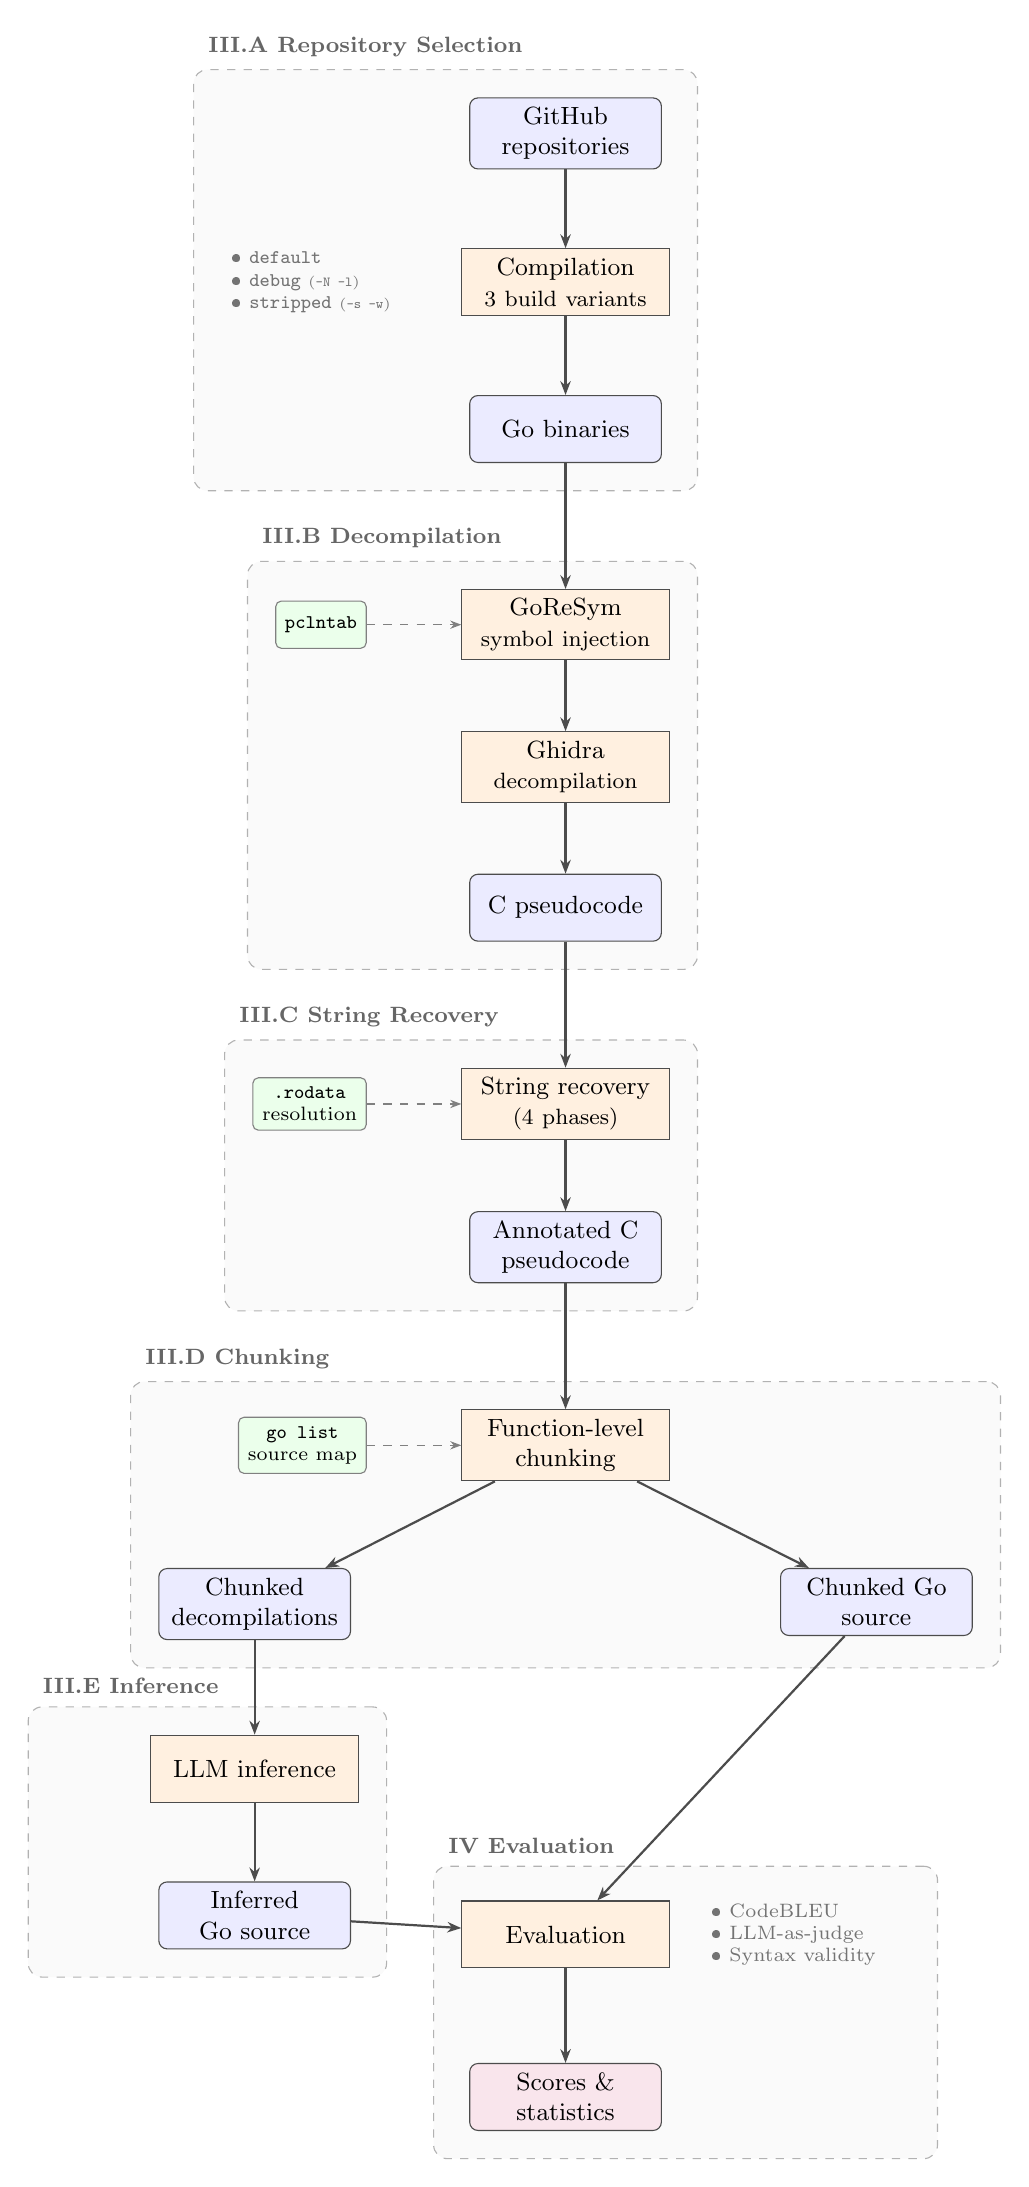
\begin{tikzpicture}[
    % Node styles
    data/.style={
        rectangle, rounded corners=3pt, draw=black!70, fill=blue!8,
        minimum width=2.4cm, minimum height=0.85cm,
        font=\small, align=center, text width=2.2cm
    },
    process/.style={
        rectangle, draw=black!70, fill=orange!12,
        minimum width=2.6cm, minimum height=0.85cm,
        font=\small, align=center, text width=2.4cm
    },
    tool/.style={
        rectangle, rounded corners=2pt, draw=black!50, fill=green!8,
        minimum height=0.6cm,
        font=\scriptsize, align=center
    },
    output/.style={
        rectangle, rounded corners=3pt, draw=black!70, fill=purple!10,
        minimum width=2.4cm, minimum height=0.85cm,
        font=\small, align=center, text width=2.2cm
    },
    arrow/.style={-{Stealth[length=5pt]}, thick, black!70},
    dasharrow/.style={-{Stealth[length=4pt]}, dashed, black!50},
    phase/.style={
        draw=black!30, dashed, rounded corners=5pt, inner sep=10pt,
        fill=gray!4
    },
    phaselabel/.style={font=\footnotesize\bfseries, black!60},
    annot/.style={font=\scriptsize, text width=2.4cm, align=left, black!55},
    node distance=1.1cm and 2.5cm
]

% ============================================================
% Central spine: data flows top to bottom
% ============================================================

% -- Section 3.1: Repository Selection & Compilation --
\node[data] (repos) {GitHub\\repositories};

\node[process, below=1.0cm of repos] (compile) {Compilation\\{\footnotesize 3 build variants}};

\node[data, below=1.0cm of compile] (binaries) {Go binaries};

\node[annot, left=0.4cm of compile] (variants) {
    \textbullet~\texttt{default}\\
    \textbullet~\texttt{debug} {\tiny(\texttt{-N -l})}\\
    \textbullet~\texttt{stripped} {\tiny(\texttt{-s -w})}
};

% -- Section 3.2: Decompilation --
\node[process, below=1.6cm of binaries] (goresym) {GoReSym\\{\footnotesize symbol injection}};

\node[process, below=0.9cm of goresym] (ghidra) {Ghidra\\{\footnotesize decompilation}};

\node[data, below=0.9cm of ghidra] (rawpseudo) {C pseudocode};

\node[tool, left=1.2cm of goresym] (pclntab) {\texttt{pclntab}};

% -- Section 3.3: String Recovery --
\node[process, below=1.6cm of rawpseudo] (strings) {String recovery\\{\footnotesize(4 phases)}};

\node[data, below=0.9cm of strings] (pseudocode) {Annotated C\\pseudocode};

\node[tool, left=1.2cm of strings] (rodata) {\texttt{.rodata}\\resolution};

% -- Section 3.4: Chunking --
\node[process, below=1.6cm of pseudocode] (chunk) {Function-level\\chunking};

% Two outputs side by side
\node[data, below left=1.1cm and 1.4cm of chunk] (chunked_decomp) {Chunked\\decompilations};
\node[data, below right=1.1cm and 1.4cm of chunk] (chunked_src) {Chunked Go\\source};

\node[tool, left=1.2cm of chunk] (golist) {\texttt{go list}\\source map};

% -- Section 4.1: Inference --
\node[process, below=1.2cm of chunked_decomp] (inference) {LLM inference};
\coordinate (p5pad) at ([xshift=-1.2cm]inference.west);

\node[data, below=1.0cm of inference] (inferred) {Inferred\\Go source};

% -- Section 4.2: Evaluation --
% Center evaluation between inferred and chunked_src
\coordinate (eval_center) at ($(inferred.south)!0.5!(chunked_src.south) + (0,-1.8)$);
\node[process] at (eval_center) (eval) {Evaluation};

\node[output, below=1.2cm of eval] (scores) {Scores \&\\statistics};

\node[annot, right=0.4cm of eval] (metrics) {
    \textbullet~CodeBLEU\\
    \textbullet~LLM-as-judge\\
    \textbullet~Syntax validity
};

% ============================================================
% Arrows
% ============================================================

% Section 3.1
\draw[arrow] (repos) -- (compile);
\draw[arrow] (compile) -- (binaries);

% 3.1 -> 3.2
\draw[arrow] (binaries) -- (goresym);

% Section 3.2
\draw[arrow] (goresym) -- (ghidra);
\draw[arrow] (ghidra) -- (rawpseudo);
\draw[dasharrow] (pclntab) -- (goresym);

% 3.2 -> 3.3
\draw[arrow] (rawpseudo) -- (strings);

% Section 3.3
\draw[arrow] (strings) -- (pseudocode);
\draw[dasharrow] (rodata) -- (strings);

% 3.3 -> 3.4
\draw[arrow] (pseudocode) -- (chunk);

% Section 3.4
\draw[arrow] (chunk) -- (chunked_decomp);
\draw[arrow] (chunk) -- (chunked_src);
\draw[dasharrow] (golist) -- (chunk);

% 3.4 -> 4.1
\draw[arrow] (chunked_decomp) -- (inference);

% 4.1 -> 4.2
\draw[arrow] (inference) -- (inferred);

% Both inputs into evaluation
\draw[arrow] (inferred) -- (eval);
\draw[arrow] (chunked_src) -- (eval);

% Evaluation output
\draw[arrow] (eval) -- (scores);

% ============================================================
% Phase bounding boxes
% ============================================================

\begin{scope}[on background layer]
    \node[phase, fit=(repos)(compile)(binaries)(variants)] (p1) {};
    \node[phase, fit=(goresym)(ghidra)(rawpseudo)(pclntab)] (p2) {};
    \node[phase, fit=(strings)(pseudocode)(rodata)] (p3) {};
    \node[phase, fit=(chunk)(chunked_decomp)(chunked_src)(golist)] (p4) {};
    \node[phase, fit=(inference)(inferred)(p5pad)] (p5) {};
    \node[phase, fit=(eval)(scores)(metrics)] (p6) {};
\end{scope}

% Phase labels — just above each box, left-aligned
\node[phaselabel, anchor=south west] at ([xshift=2pt, yshift=1pt]p1.north west)
    {III.A Repository Selection};
\node[phaselabel, anchor=south west] at ([xshift=2pt, yshift=1pt]p2.north west)
    {III.B Decompilation};
\node[phaselabel, anchor=south west] at ([xshift=2pt, yshift=1pt]p3.north west)
    {III.C String Recovery};
\node[phaselabel, anchor=south west] at ([xshift=2pt, yshift=1pt]p4.north west)
    {III.D Chunking};
\node[phaselabel, anchor=south west] at ([xshift=2pt, yshift=1pt]p5.north west)
    {III.E Inference};
\node[phaselabel, anchor=south west] at ([xshift=2pt, yshift=1pt]p6.north west)
    {IV Evaluation};

\end{tikzpicture}

\end{document}
